\documentclass[sigplan,screen,nonacm]{acmart}
\usepackage{tikz}
\usetikzlibrary{shapes, arrows, positioning}
\raggedbottom

\settopmatter{printacmref=false} % Removes ACM Reference Format
\setcopyright{none} % Removes copyright info
\renewcommand\footnotetextcopyrightpermission[1]{} % Removes footnote with conference info

%%
%% \BibTeX command to typeset BibTeX logo in the docs
\AtBeginDocument{%
  \providecommand\BibTeX{{%
    Bib\TeX}}}

%% Rights management information.
\setcopyright{none}
%\copyrightyear{2025}
%\acmYear{2025}
%\acmDOI{XXXXXXX.XXXXXXX}

%% These commands are for a PROCEEDINGS abstract or paper.
\pagestyle{plain}
\begin{document}

\title{Darknet Duel}
\subtitle{A Cybersecurity-Themed Card Game}

\author{Matthew Emmanuel O. Echavez}
\affiliation{%
  \institution{Cebu Institute of Technology - University}
  \city{Cebu City}
  \country{Philippines}
}
\email{matthewemmanuel.echavez@cit.edu}

\author{Brian Steve E. Pila}
\affiliation{%
  \institution{Cebu Institute of Technology - University}
  \city{Cebu City}
  \country{Philippines}
}
\email{briansteve.pila@cit.edu}

\author{Ephraim Jay A. Solasco}
\affiliation{%
  \institution{Cebu Institute of Technology - University}
  \city{Cebu City}
  \country{Philippines}
}
\email{ephraimjay.solasco@cit.edu}

\author{Kenjie B. Bentain}
\affiliation{%
  \institution{Cebu Institute of Technology - University}
  \city{Cebu City}
  \country{Philippines}
}
\email{kenjie.bentain@cit.edu}

\author{Scott Benzer Gitgano}
\affiliation{%
  \institution{Cebu Institute of Technology - University}
  \city{Cebu City}
  \country{Philippines}
}
\email{scottbenzer.gitgano@cit.edu}

\author{Eugene C. Busico}
\affiliation{%
  \institution{Cebu Institute of Technology - University}
  \city{Cebu City}
  \country{Philippines}
}
\email{eugene.busico@cit.edu}

\renewcommand{\shortauthors}{Echavez et al.}

\begin{abstract}
    Traditional cybersecurity education often fails to engage learners, leading to poor retention of critical concepts. To address this, we present \textit{Darknet Duel}, a multiplayer web-based card game designed to gamify cybersecurity awareness. Built using a modern technology stack including React, Node.js, and Boardgame.io, the system ensures a responsive and scalable gaming experience. We conducted rigorous performance testing, demonstrating the server's ability to handle over 176 concurrent users. User evaluation involving 33 participants yielded a System Usability Scale (SUS) score of 50.9. While participants praised the game's concept and visual design, results indicate a need for improved onboarding to address the steep learning curve. This paper details the design, implementation, and evaluation of Darknet Duel, highlighting its potential as an engaging educational tool and outlining future improvements.
\end{abstract}

\begin{CCSXML}
    <ccs2012>
    <concept>
    <concept_id>10002978.10003029.10011703</concept_id>
    <concept_desc>Security and privacy~Usability in security and privacy</concept_desc>
    <concept_significance>500</concept_significance>
    </concept>
    <concept>
    <concept_id>10002978.10003022.10003028</concept_id>
    <concept_desc>Security and privacy~Social aspects of security and privacy</concept_desc>
    <concept_significance>300</concept_significance>
    </concept>
    <concept>
    <concept_id>10010405.10010489.10010491</concept_id>
    <concept_desc>Applied computing~Interactive learning environments</concept_desc>
    <concept_significance>500</concept_significance>
    </concept>
    </ccs2012>
\end{CCSXML}

\ccsdesc[500]{Security and privacy~Usability in security and privacy}
\ccsdesc[300]{Security and privacy~Social aspects of security and privacy}
\ccsdesc[500]{Applied computing~Interactive learning environments}

\keywords{Cybersecurity, Gamification, Card Game, Education, Awareness}

\maketitle

\section{Introduction}
The increasing reliance on digital technologies has highlighted the importance of cybersecurity awareness. A significant section of the population is still unaware of the basic risks that the online world poses. Due to the fact that people make mistakes, fail to see potential dangers, and lack understanding of cybersecurity, people are often considered the weakest link in computer security and are therefore susceptible to cyberattacks.

Traditional learning resources are available, but they usually fail to maintain students' attention, which leads to inadequate understanding and recall of cybersecurity fundamentals. Students typically don't participate in traditional teaching techniques like lectures and textbooks, which results in poor material recall. Additionally, most of the gamified learning materials available today fall short of the goal because they are either too easy or too difficult, which keeps users from receiving a sufficient education.

To address this gap, we propose \textit{Darknet Duel}, a gamified web-based card game designed to teach cybersecurity awareness in a strategic, engaging, and fun way. The game pits attackers against defenders, each using cards that represent ways of attacking, defending, and real-world cybersecurity events. By combining fast-paced gameplay with educational elements, Darknet Duel simplifies the concepts of cybersecurity while keeping users entertained.

\section{Related Work}
Gamification has emerged as a powerful strategy for enhancing cybersecurity awareness and education. This section reviews relevant literature on the effectiveness of gamification and analyzes existing solutions to identify gaps that Darknet Duel aims to address.

\subsection{Gamification in Cybersecurity Education}
Research consistently demonstrates the positive impact of gamification on engagement and knowledge retention. Institutions like the Berkeley Center for Long-Term Cybersecurity have highlighted the transformative potential of gamification in education \cite{berkeley}. Similarly, industry insights suggest that gamification is crucial for effective security awareness training, as it significantly boosts learner motivation \cite{inspired}.

Scholefield and Shepherd explored the use of gamification for password security education, developing an RPG for Android. Their findings indicated that participants enjoyed the interactive learning experience, suggesting that gamified methods can effectively meet educational needs \cite{scholefield2019}. Studies on learning effectiveness further support this, showing that security awareness through gaming can lead to better educational outcomes \cite{ijcic}.

Addressing the issue of knowledge deterioration, Fatokun et al. investigated gamification as an intervention strategy. Their study found that gamified learning opportunities could serve as a proactive measure to maintain high levels of user awareness and reinforce cybersecurity expertise, countering the tendency for knowledge to fade over time \cite{fatokun2024}.

Williams et al. focused on students with no prior knowledge, using game mechanics to demystify difficult cybersecurity concepts. They discovered that elements like storytelling and puzzles not only raised interest but also improved comprehension and memory of the subject matter \cite{williams2024}. Similarly, Nwokeji et al. found that information systems students exposed to a gamified curriculum showed greater engagement and deeper understanding compared to those receiving standard instruction \cite{nwokeji2020}.

Furthermore, a systematic review by Gwenhure and Rahayu highlighted the effectiveness of gamification for non-IT professionals, a group often disengaged by conventional training. They concluded that gamification helps bridge the gap between technical material and non-technical audiences, fostering a security-conscious culture \cite{gwenhure2024}.

\subsection{Existing Solutions}
Despite the theoretical support for gamification, existing implementations often have limitations.

Byte Club Cybersecurity Card Game is a physical card-based game with a focus on cybersecurity education and strategic elements \cite{byteclub}. While it has an established brand and proven educational value, its physical nature limits its accessibility compared to a web-based platform. It is also not free to play, creating a cost barrier. Darknet Duel disrupts this by offering a web-based, multiplayer experience that is easily accessible.

Cyber Threat Defender is a multiplayer card game with collectible elements \cite{ctd}. While effective, its reliance on deck-building and strategic depth similar to complex TCGs can present a steeper learning curve for casual players compared to Darknet Duel's streamlined mechanics.

Cyber Awareness Challenge focuses on education for government and military personnel \cite{cac}. However, it suffers from an outdated design and lack of interactivity, often relying on lengthy videos. Darknet Duel improves upon this by providing a modern, interactive, and engaging learning experience.

\section{Methodology}
\subsection{System Architecture}
Darknet Duel is built as a modern web application using a robust technology stack designed for performance, scalability, and user experience.

\begin{figure}[h]
    \centering
    \resizebox{\columnwidth}{!}{%
    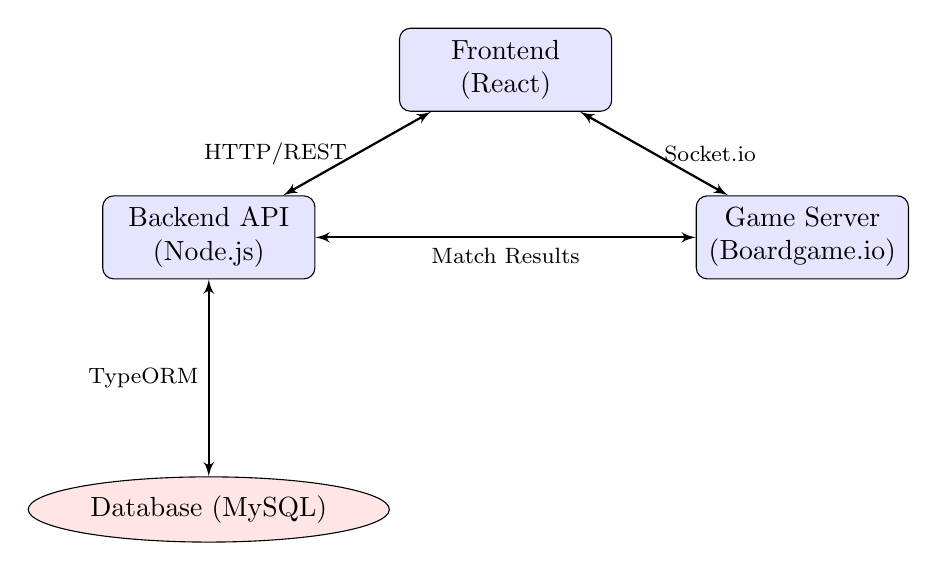
\begin{tikzpicture}[
        node distance=1.5cm,
        auto,
        block/.style={
            rectangle,
            draw,
            fill=blue!10,
            text width=7em,
            text centered,
            rounded corners,
            minimum height=3em
        },
        cloud/.style={
            draw,
            ellipse,
            fill=red!10,
            node distance=2.5cm,
            minimum height=2em
        },
        line/.style={
            draw,
            -latex',
            thick
        },
        dbl/.style={
            draw,
            latex'-latex',
            thick
        }
    ]
        % Nodes
        \node [block] (frontend) {Frontend (React)};
        \node [block, below left=of frontend] (backend) {Backend API (Node.js)};
        \node [block, below right=of frontend] (gameserver) {Game Server (Boardgame.io)};
        \node [cloud, below=of backend] (db) {Database (MySQL)};

        % Paths
        \path [dbl] (frontend) -- node [left, font=\footnotesize] {HTTP/REST} (backend);
        \path [dbl] (frontend) -- node [right, font=\footnotesize] {Socket.io} (gameserver);
        \path [dbl] (backend) -- node [left, font=\footnotesize] {TypeORM} (db);
        \path [dbl] (backend) -- node [below, font=\footnotesize] {Match Results} (gameserver);
        
    \end{tikzpicture}%
    }
    \caption{High-Level System Architecture}
    \label{fig:architecture}
\end{figure}

\subsubsection{Frontend}
The user interface is built using React, a popular JavaScript library for building user interfaces. We utilize Vite as the build tool for its fast development server and optimized production builds. For styling, we employ TailwindCSS and DaisyUI to create a modern, responsive, and visually appealing design that enhances the gaming experience.

\subsubsection{Backend API}
The backend API is developed using Node.js and Express, providing a flexible and scalable server environment. We use TypeScript to ensure type safety and code maintainability. Data persistence is managed by MySQL, with TypeORM serving as the Object-Relational Mapper (ORM) to interact with the database efficiently. Authentication is handled via server-side sessions, which allows for granular control over user access, including the ability to invalidate sessions for logging out or banning users.

\subsubsection{Game Server}
To manage the real-time multiplayer state, we utilize Boardgame.io. This framework simplifies the development of turn-based games by handling state management, move validation, and synchronization between clients. Communication between the client and the game server is facilitated by Socket.io, ensuring low-latency updates during gameplay.

\subsection{Justification}
The choice of React allows for a dynamic and responsive UI, essential for a card game. Node.js and Express provide a lightweight yet powerful backend capable of handling concurrent requests. Boardgame.io was selected specifically for its specialized features for turn-based games, reducing the complexity of implementing game logic and state synchronization from scratch.

\section{Implementation}
\subsection{Development Model}
We adopted the Waterfall Model for the development of Darknet Duel. This structured approach allowed us to have a stable development lifecycle, ensuring that each phase---from requirements gathering to design, implementation, and testing---was completed before moving to the next. This was particularly beneficial for defining the game rules and mechanics clearly before writing code.

\subsection{Deployment and DevOps}
To ensure consistent environments and ease of deployment, we utilized Docker to containerize both the frontend and backend applications. This eliminates "it works on my machine" issues and simplifies dependency management.

For Continuous Integration and Continuous Deployment (CI/CD), we implemented GitHub Actions. This automated pipeline runs tests and builds the Docker images whenever changes are pushed to the repository, ensuring code quality and rapid feedback.

The application is deployed on a DigitalOcean server (Droplet). The Docker containers are orchestrated to run the web server, API server, and database on the cloud infrastructure, making the game accessible to users over the internet.

\section{Performance Testing}
Before deploying the application, we conducted rigorous performance testing to evaluate the server's capacity and stability under load.

\subsection{Test Environment}
The server environment consisted of a quad-core AMD Ryzen 3 5300U processor with 20GB of RAM, running Ubuntu Server. This setup was chosen to simulate a realistic hosting environment for a medium-scale web application.

\subsection{Methodology}
We developed a custom Node.js script to simulate multiple users performing concurrent API calls. Each simulated user executed seven specific API calls simultaneously, representing the most common actions a real user would perform:
\begin{itemize}
    \item \textbf{Lobby:} Browsing the lobby list and creating a new lobby.
    \item \textbf{Login:} Authenticating with the server.
    \item \textbf{Profile:} Retrieving user profile data.
    \item \textbf{Register:} Creating a new user account.
    \item \textbf{Search:} Searching for other users.
    \item \textbf{Socket:} Initiating a game session and simulating moves.
    \item \textbf{Update:} Updating profile information.
\end{itemize}

The test started with a single user and incrementally added $n+1$ users. The script was designed to automatically halt if any endpoint failed to respond within a maximum tolerable threshold of 5000ms.

\subsection{Results}
The stress test successfully handled a load of 176 concurrent users. The latency remained within acceptable limits until the 177th user was added, at which point a random ping spike on an API endpoint caused the response time to exceed the 5000ms threshold, halting the script.

\begin{figure}[h]
    \centering
    \includegraphics[width=\linewidth]{../../performance-tests/images/max_users_graph.png}
    \caption{Maximum Concurrent Users}
    \label{fig:max_users}
\end{figure}

Extrapolating from the data collected, the server could theoretically handle up to 286 concurrent users before reaching critical failure points, assuming ideal conditions.

\begin{figure}[h]
    \centering
    \includegraphics[width=\linewidth]{../../performance-tests/images/latency_breakdown.png}
    \caption{Latency Breakdown by Endpoint}
    \label{fig:latency}
\end{figure}

Analysis of the 177th run revealed that the \textbf{Register} endpoint experienced the highest latency. This is consistent with expectations, as registration involves a write operation to the database, which is inherently more resource-intensive than read operations.

It is important to note that this test assumes a "worst-case" scenario where every user is placing maximum load on the server simultaneously. In a real-world scenario, user activity would likely be more distributed, suggesting that the server could theoretically handle a higher number of active users than the stress test indicates.

\section{Results and Evaluation}
To evaluate the usability and effectiveness of Darknet Duel, we conducted a System Usability Scale (SUS) test with 33 college student respondents within Cebu Institute of Technology - University within a one-day period.

\subsection{SUS Results}
The average SUS score calculated from the participant responses is 50.9. According to standard SUS interpretation, this score falls into the "Marginal" or "Low" acceptability range. While some users found the system easy to use and integrated well, others reported challenges with complexity and learning the game mechanics.

\subsection{Qualitative Feedback}
We also collected open-ended feedback to understand user sentiments better. Participants praised the User Interface (UI) and the concept of the game. Many found the idea of learning cybersecurity through a card game to be "fun," "unique," and "educational." The visual design and animations were also highlighted as positive aspects.

However, the primary challenge reported by users was the complexity of the game mechanics and the steep learning curve. Several users mentioned that the tutorial had bugs or was not sufficient to fully understand the game. A specific issue was raised regarding pop-up cards blocking the view of important details during the tutorial and gameplay.

To address these issues, users suggested improving the tutorial to be more comprehensive and bug-free. Visual cues, such as clearer indicators for whose turn it is and better highlighting of interactive elements, were also requested. Some users expressed a desire for a "practice mode" against an AI opponent before playing against real people.

\section{Conclusion}
Darknet Duel represents a significant step towards making cybersecurity education more accessible and engaging. By gamifying complex concepts, we have created a platform that appeals to a broad audience.

While the initial evaluation shows promise in terms of concept and design, the SUS score of 50.9 indicates that there is significant room for improvement in terms of usability and learnability. The feedback highlights the need for a more robust tutorial and a simplified onboarding process.

Moving forward, we plan to address these issues by refining the game mechanics, fixing the reported bugs in the tutorial, and enhancing the visual feedback system. We believe that with these improvements, Darknet Duel can become a highly effective tool for raising cybersecurity awareness.

\begin{acks}
    We would like to thank our test participants for their valuable feedback.
\end{acks}

\bibliographystyle{ACM-Reference-Format}
\begin{thebibliography}{9}
    
    \bibitem{berkeley}
    Berkeley Center for Long-Term Cybersecurity.
    \textit{Gamification of Cybersecurity Education}.
    Retrieved from \url{https://cltc.berkeley.edu/publication/gamification-of-cybersecurity-education}
    
    \bibitem{inspired}
    Inspired eLearning.
    \textit{The Importance of Gamification in Security Awareness Training}.
    Retrieved from \url{https://inspiredelearning.com/blog/gamification-importance-security-awareness-training}

    \bibitem{scholefield2019}
    Scholefield, S., \& Shepherd, L. A. (2019).
    Gamification Techniques for Raising Cyber Security Awareness.
    \textit{SpringerLink}.
    Retrieved from \url{https://link.springer.com/chapter/10.1007/978-3-030-22351-9_13}
    
    \bibitem{ijcic}
    International Journal of Cybersecurity Intelligence \& Cybercrime.
    \textit{Security Awareness Through Gaming: A Study on Learning Effectiveness}.
    Retrieved from \url{https://sites.asee.org/se/wp-content/uploads/sites/56/2021/01/2020ASEESE117.pdf}

    \bibitem{fatokun2024}
    Faith Fatokun, Zalizah Awang, Suraya Hamid, Johnson O. Fatokun, \& Azah Norman. (2024).
    Cybersecurity knowledge deterioration and the role of gamification intervention.
    \textit{Journal of Advanced Research in Applied Sciences and Engineering Technology}, 43(1), 66–94.
    \url{https://doi.org/10.37934/araset.43.1.6694}
    
    \bibitem{williams2024}
    Williams, L., Anthi, E., Cherdantseva, Y., \& Javed, A. (2024).
    Leveraging gamification and game-based learning in Cybersecurity Education.
    \textit{Journal of The Colloquium for Information Systems Security Education}, 11(1), 8.
    \url{https://doi.org/10.53735/cisse.v11i1.186}

    \bibitem{nwokeji2020}
    Nwokeji, J. C., Matovu, R., \& Rawal, B. (2020).
    The Use of Gamification to Teach Cybersecurity Awareness in Information Systems.
    Retrieved from \url{https://www.researchgate.net/publication/349917575}
    
    \bibitem{gwenhure2024}
    Gwenhure, A. K., \& Sapty Rahayu, F. (2024).
    Gamification of cybersecurity awareness for Non-IT Professionals: A Systematic Literature Review.
    \textit{International Journal of Serious Games}, 11(1), 83–99.
    \url{https://doi.org/10.17083/ijsg.v11i1.719}

    \bibitem{byteclub}
    CyberSec Games.
    \textit{Byte Club Cybersecurity Card Game}.
    Retrieved from \url{https://www.cybersecgames.com}

    \bibitem{ctd}
    Center for Infrastructure Assurance and Security (CIAS).
    \textit{Cyber Threat Defender}.
    Retrieved from \url{https://cias.utsa.edu/ctd/}

    \bibitem{cac}
    Department of Defense Cyber Exchange.
    \textit{Cyber Awareness Challenge}.
    Retrieved from \url{https://public.cyber.mil/training/cyber-awareness-challenge/}
    
\end{thebibliography}

\end{document}
